% Specify the type of document
\documentclass[12pt]{article}

% Load a number of useful packages
\usepackage{graphicx}
\usepackage{amsmath,amssymb,amsfonts,amsthm}
 \usepackage[margin=1.0in]{geometry}
\usepackage[colorlinks=true]{hyperref}
\usepackage{cite}
\usepackage[caption=false,font=footnotesize]{subfig}
\usepackage{listings}
\usepackage{tikz}

\DeclareMathOperator*{\minimize}{minimize} 
\providecommand{\norm}[1]{\left\lVert#1\right\rVert}

% Say where pictures (if any) will be placed
\graphicspath{{./pictures/}}

% Define title, author, and date
\title{598RL: HW \#1}
\author{T. Bretl \and M. West}
\date{(due by 10AM on Thursday, September 6)}

% Start of document
\begin{document}

% Put the title, author, and date at top of first page
\maketitle


\section{A pursuit-evasion game}

Consider the $4\times4$ grid with boundary that is shown in Figure \ref{fig:pursuit}. You control the good robot (blue circle). At each time step, the good robot can stay in the same place or can move one cell north, south, east, or west. The good robot cannot move through the boundary (i.e., out of the grid)---if it tries, the result is to stay in the same place. The evil robot (red triangle) has a mind of its own. At each time step, the evil robot either stays in the same place (20\% chance) or moves one cell in a direction chosen at random (20\% north, south, east, or west). Like the good robot, the evil robot cannot move through the boundary---if it tries, it stays in the same place. The good robot would like to spend as much time at the goal (green square) as possible. This goal has a fixed location. If the good robot ends a time step in the same cell as goal, it receives a reward of +1. If the good robot instead ends a time step in the same cell as the evil robot, the game is over. Each time the game is played, the good robot, the bad robot, and the goal are each chosen uniformly at random (so, it is possible for a game to have length zero). The good robot knows its own location as well as the location of both the bad robot and the goal at each time step.
\begin{itemize}
\item Formulate this game as an MDP.
\item Write python code that\ldots
\item Visualize an example game\ldots
\end{itemize}

\begin{figure}[htbp]
\begin{center}
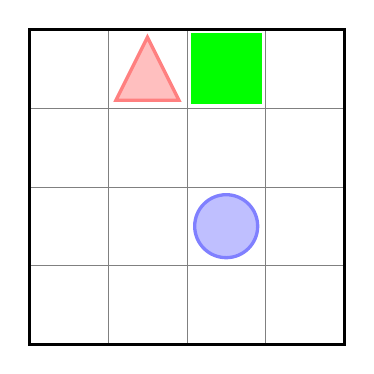
\begin{tikzpicture}
\newcommand\GoalShape[1]{+(-#1,-#1) rectangle +(#1,#1)}
\newcommand\HazardShape[1]{+(-#1, -#1) -- +(#1, -#1) -- +(0, #1) -- cycle}
\draw[step=1cm, gray, very thin, shift={(-0.5, -0.5)}] (0, 0) grid (4, 4);
\draw[very thick, shift={(-0.5, -0.5)}] (0,0) rectangle (4,4);
\draw[color=blue!50, fill=blue!25, very thick] (2, 1) circle (0.4cm);
\fill[green!100!white] (2,3) \GoalShape{0.45cm};
\draw[color=red!50, fill=red!25, very thick] (1, 3) \HazardShape{0.4cm};
\end{tikzpicture}
\caption{The playing field for a game of pursuit-evasion.}
\label{fig:pursuit}
\end{center}
\end{figure}







% End of document (everything after this is ignored)
\end{document}